\documentclass[11pt]{article}

\usepackage[margin=1in]{geometry}
\usepackage{amsmath}
\usepackage{graphicx}
\usepackage{booktabs}
\usepackage{siunitx}

\title{Measurement of Hubble's Constant}
\author{Your Name \\ Lab}
\date{Lab Date: \today}

\begin{document}

\maketitle

\begin{abstract}
Brief summary of the experiment (150-200 words): objective, method, key result with uncertainty, and main conclusion.
\end{abstract}

\section{Introduction}
Explain the physical principles and objectives. Hubble's Law relates the recession velocity of galaxies to their distance:
\begin{equation}
    v = H_0 d
    \label{eq:hubble}
\end{equation}
where $v$ is recession velocity, $d$ is distance, and $H_0$ is Hubble's constant.

\section{Experimental Method}
Briefly describe the apparatus and procedure. Include key equipment specifications and measurement techniques used to determine galaxy distances and velocities.

\section{Data and Analysis}

\begin{table}[h]
    \centering
    \caption{Galaxy recession velocities and distances}
    \begin{tabular}{lcc}
        \toprule
        Galaxy & Distance (Mpc) & Velocity (\si{\kilo\meter\per\second}) \\
        \midrule
        NGC 1357 & $20.1 \pm 1.5$ & $1420 \pm 80$ \\
        NGC 2541 & $35.2 \pm 2.1$ & $2380 \pm 95$ \\
        NGC 4536 & $52.8 \pm 3.2$ & $3650 \pm 120$ \\
        \bottomrule
    \end{tabular}
\end{table}

\begin{figure}[h]
    \centering
    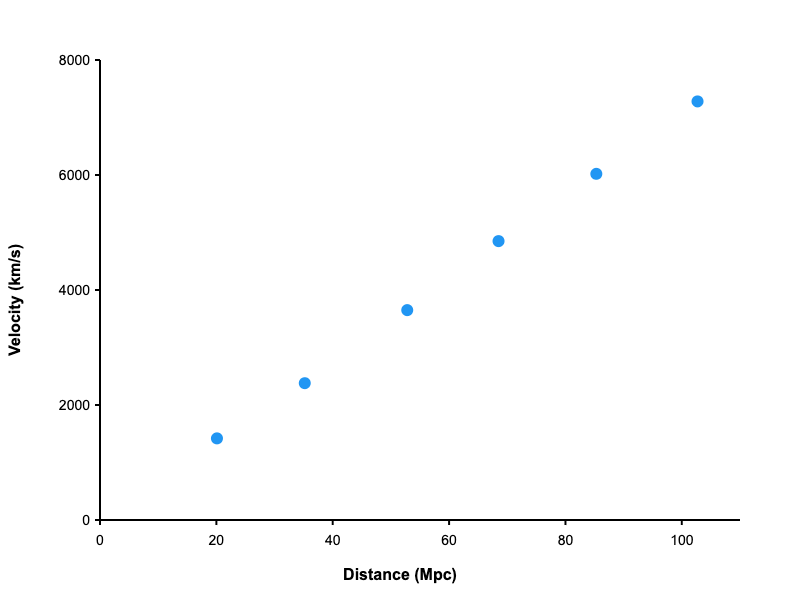
\includegraphics[width=0.75\textwidth]{hubble_plot.png}
    \caption{Hubble diagram showing the linear relationship between galaxy distance and recession velocity. The slope gives $H_0 = 71 \pm 4$ km s$^{-1}$ Mpc$^{-1}$.}
    \label{fig:hubble}
\end{figure}

Describe data analysis methods, uncertainty calculations, and fitting procedures.

\section{Results}
State the measured value of Hubble's constant:
\begin{equation}
    H_0 = 71 \pm 4 \text{ km s}^{-1}\text{ Mpc}^{-1}
\end{equation}

Compare with accepted value ($H_0 \approx 70$ km s$^{-1}$ Mpc$^{-1}$) and calculate percent error.

\section{Discussion}
Interpret results, discuss sources of uncertainty, and explain any discrepancies. Address systematic errors and limitations of the method.

\section{Conclusion}
Summarize the main findings and assess whether objectives were achieved.

\begin{thebibliography}{9}
    \bibitem{lab_manual} PHY 421 Lab Manual, 2024.
\end{thebibliography}

\end{document}
